\section{Intersection Computation}

\label{section:isect}
%In this step, intersections between faces are computed through triangle-triangle intersection test. We adopt M\"{o}ller's algorithm \cite{moller1997fast} on account of its efficiency and simplicity. However, a naive implementation of M\"{o}ller's algorithm can introduce numerical errors and may fail to produce correct results. Therefore, we integrate plane-based geometry to make it exact. In the following, we first introduce our space division strategy to reduce the number of intersection test. Then we make a quick review of M\"{o}ller's algorithm, and discuss the way to embed plane-based geometry. After that, we discuss how to deal with degenerate cases.

In this step, the intersections between faces are determined by a triangle-triangle intersection test. We use  M\"{o}ller's algorithm \cite{moller1997fast} because of its efficiency and simplicity. To ensure exact intersection computation, we integrate P-rep based geometry into the algorithm. In the following, we first introduce our space division strategy to reduce the number of intersection tests. Then introduce our P-rep based intersection algorithm. Lastly, we discuss how to deal with degenerate cases.

\subsection{Space Division}
\begin{wrapfigure}{r}[0in]{0in}
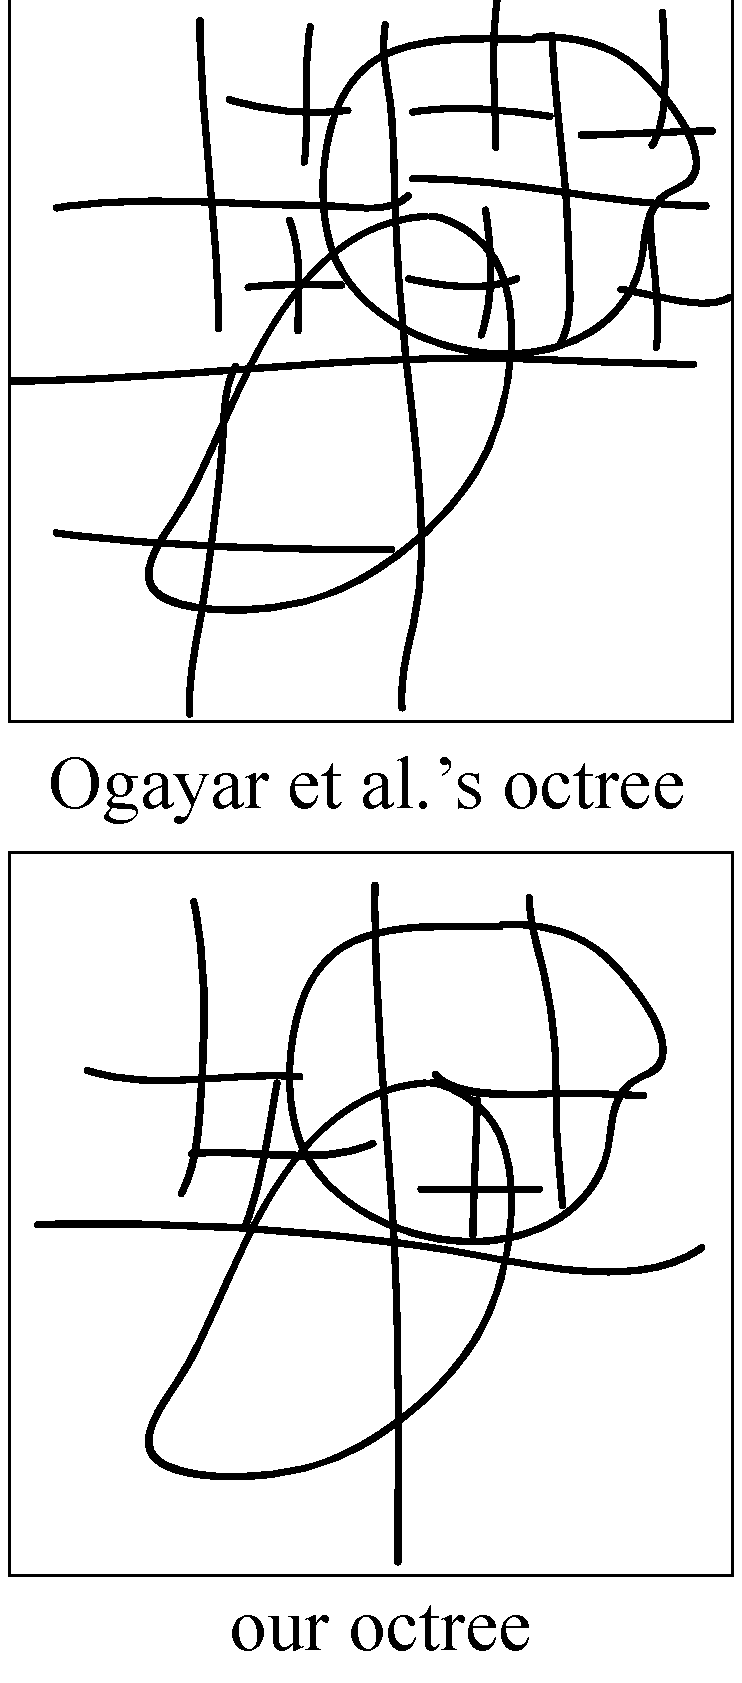
\includegraphics[width=1.2in]{octreediff}
\end{wrapfigure}


%As intersection detection is performed between each pair of faces, localization is necessary for large CSGs to reduce the number of testing pairs. We use the adaptive octree for this purpose. Our implementation is akin to the implementation in Ogayar et al.'s method \cite{ogayar2015deferred}. Intersection between triangle faces and octree nodes are efficiently detected using the separating axis theorem \cite{gottschalk1996obbtree}. Octree leaves are classified into two types: if all faces that intersect a leaf belong to the same mesh, we call it a \emph{normal cell}. Otherwise, it is a \emph{critical cell}, within which the following intersection computation is performed.

As intersection detection is performed between each pair of faces, space division is necessary to reduce the number of pairs to be tested. We use an adaptive octree for this purpose. Our implementation is akin to the implementation of Ogayar et al. \cite{ogayar2015deferred}. The intersections between triangle faces and octree nodes are efficiently detected using the separating axis theorem \cite{gottschalk1996obbtree}. Octree leaves are classified into two types. If all faces that intersect a leaf belong to the same mesh, we regard it as a \emph{normal cell}. Otherwise, it is regarded as a \emph{critical cell}, within which the following intersection computation is performed.

%The difference between our octree and Ogayar et al.'s is that we do not subdivide any normal cell no matter how many faces it contains. This is because subdividing normal cells benefits only the point-in-polyhedron test \cite{frisken2002simple}, which seldom uses in our method. This simplification can save much computing time, especially when intersections between primitives are not complex and located in small regions.

The difference between our octree and that of Ogayar et al. is that we do not subdivide any normal cell, no matter how many faces it contains. Subdividing normal cells is only beneficial for the point-in-polyhedron test \cite{frisken2002simple}, which is seldom used in our method. This simplification saves significant computing time, especially when intersections between primitives are simple, and located in small regions.

\subsection{Plane-Based Intersection Test}

We first make a quick review of M\"{o}ller's V-rep based algorithm. Then we introduce our implicit representations of intersections using planes. After that, we discuss how to implement  M\"{o}ller's algorithm using P-rep based geometry.

\subsubsection{Review of M\"{o}ller's algorithm}



M\"{o}ller's algorithm computes the intersection between two triangles $t_1$ and $t_2$ in three steps as shown in Fig. \ref{fig_projection}:
\begin{itemize}[leftmargin=0.45cm]
\item[1)] An early rejection is performed by testing whether $t_1$ intersects $\bm{p}_{t_2, sp}$, the supporting plane of $t_2$. The same test is also carried out between $t_2$ and $\bm{p}_{t_1, sp}$.
\item[2)]The intersection between $t_1$ and $\bm{p}_{t_2, sp}$, denoted as $Seg_1$, and the intersection between $t_2$ and $\bm{p}_{t_1, sp}$, denoted as $Seg_2$, are computed separately.
 \item[3)]The intersection between $t_1$ and $t_2$ is determined by computing the overlap between $Seg_1$ and $Seg_2$ .
\end{itemize}



The non-robustness of this algorithm stems from computing the coordinates of the intersection vertices (the end points of $Seg_1$ and $Seg_2$). Although implementation of this algorithm with arbitrary precision arithmetic produces exact coordinates, it is too costly for boolean operations with large CSGs. We use plane-based geometry to solve this problem, by implicitly representing intersections with planes.

\subsubsection{Plane-based intersection representation}
\label{sec:ir}

In our method, the intersection with triangle $t$ is stored as $\bm{\mathcal{I}}\colon\{T, \bm{P}_{ext}, \bm{P}_0, \bm{P}_1, \mathcal{N}\}$. This is the plane-based intersection representation (PBI-rep,  see Fig. \ref{fig:pbi}). The first component, $T$, indicates which triangle $\bm{\mathcal{I}}$ lies on.
$\bm{P}_{ext}$ indicates the plane that $\bm{\mathcal{I}}$ lies on. Note that $T$ is not in $\bm{P}_{ext}$. The first two components indicate that  $\bm{\mathcal{I}}$ lies on the line $T \cap \bm{P}_{ext}$.
The two end points of $\bm{\mathcal{I}}$ are $T \cap \bm{P}_{ext}\cap\bm{P}_0$ and $T \cap \bm{P}_{ext}\cap\bm{P}_1$.
The last component, $\mathcal{N}$, represents the neighborhood faces of $\bm{\mathcal{I}}$. $\mathcal{N}$ can be a single face, or a set faces from different input primitives.

\begin{figure}[t]
\centering
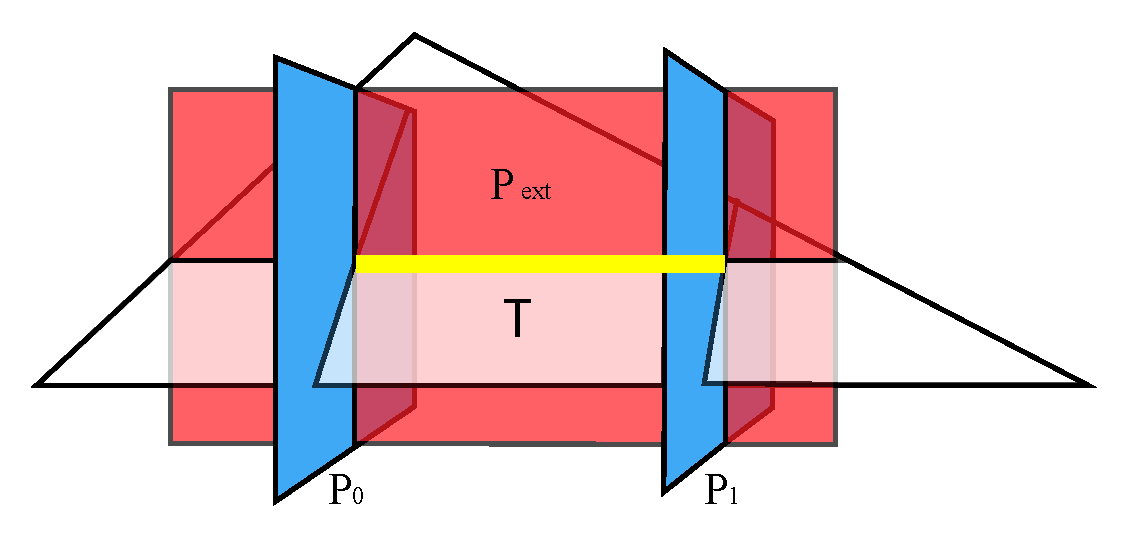
\includegraphics[width=3in]{pbirep2}
\caption{The geometry of planes in a PBI-rep. The yellow line segment is the intersection represented by $\bm{\mathcal{I}}$.}
\label{fig:pbi}
\end{figure}

For example, two triangle faces, $t_1$ and $t_2$, originating from meshes $M_i$ and $M_j$, respectively, intersect. Two intersections are generated, ${\bm{\mathcal{I}}}_{12}$ on $t_1$ and ${\bm{\mathcal{I}}}_{21}$ on $t_2$.
For ${\bm{\mathcal{I}}}_{12}$, $T = t_1$ and $\bm{P}_{ext}=\bm{p}_{t_2, sp}$. $\bm{P}_0$ and $\bm{P}_1$ are boundary planes of $t_2$, which will be discussed later.
The last component $\mathcal{N}=t_2$ in general situation. Sometimes, ${\bm{\mathcal{I}}}_{12}$ may lie on the edge of $t_2$ (see Fig. \ref{fig:twin}). This is called \emph{edge intersection}. In this situation, the $\mathcal{N}$ is the set of all faces from $M_j$ adjacent to that edge. Edge intersection is discussed in \S\ref{sec:degenerate}.


\subsubsection{Plane-based implementation}

\label{sec:embed}
\begin{figure}[t]
\centering
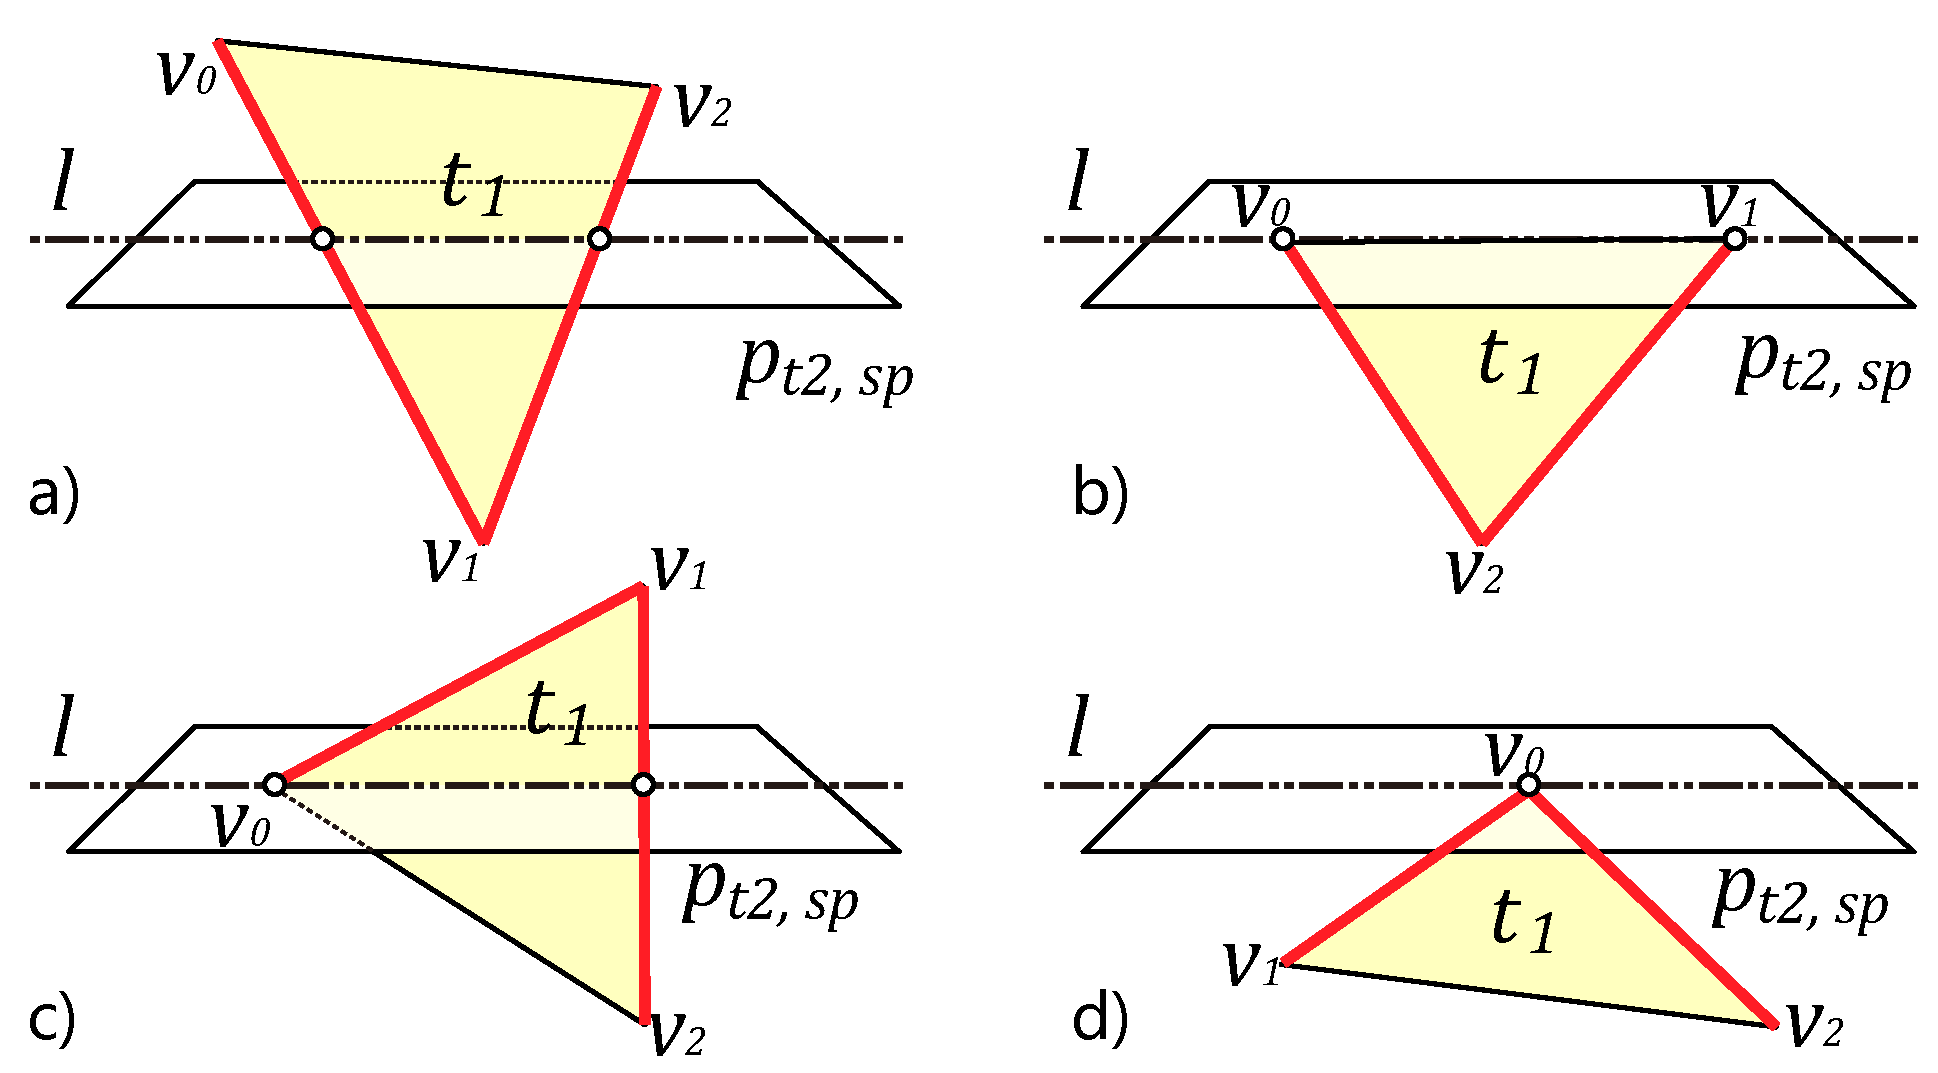
\includegraphics[width=3.5in]{sign}
\caption{We denote the signed distance from point $v_i$ to plane $\bm{p}_{t_2, sp}$ as $d_i$. The four conditions of intersection between $t_1$ and $\bm{p}_{t_2, sp}$ are:
(a) $d_0\cdot d_2<0$, $d_1\cdot d_2<0$;
(b) $d_0=0$, $d_1=0$, $d_2\neq 0$;
(c) $d_0=0$, $d_1\cdot d_2<0$;
(d) $d_0=0$, $d_1\cdot d_2>0$. End points of $Seg_1$ are the intersections between $\bm{p}_{t_2, sp}$ and the related edges of $t_1$ (bold red lines).}
\label{fig:isect}
\end{figure}

To implement M\"{o}ller's algorithm by plane-based geometry, we first convert each triangle to its P-reps: a supporting plane $\bm{p}_{t, sp}$  surrounded by three bounding planes $\{\bm{p}_{t, b}^i|\ i = 0,1,2\}$. The substrates of the intersection algorithms are point-plane orientation \cite{bernstein2009fast} and linear order of points (\S\ref{sec:substrates}), both of which can be implemented by plane-based geometry.

In the first step, the computation of signed distances involves only the vertices coordinates and the supporting planes of triangles. Therefore, if the early rejections occur, the bounding planes are not needed at all. In addition, according to the conversion method of Campen et al.\cite{campen2010exact}, the supporting plane is represented by four double precision floating point numbers. The precision of first three parameter $L_a$ and the precision of the last parameter $L_d$ hold the relation $L_d = L_a + L + 1$, where $L$ is the precision of coordinates of input vertices. This means we can compute the signed distance exactly within double-precision. With these two facts, our early rejection is as fast as the vertex-based implementation.

If $t_1$ and $t_2$ are not coplanar, $Seg_1$ and $Seg_2$ are computed. The end points are intersections between the supporting plane of one triangle and an edge of the other triangle. By computing the bounding planes, the end points can be implicitly represented by plane triples, $\bm{p}_{t_2, sp} \cap \bm{p}_{t_1, sp} \cap \bm{p}^i_{t_1, b}$, where $\bm{p}^i_{t_1, b}$ is the bounding plane of the related edge.
Fig. \ref{fig:isect} shows all of the possible intersection conditions between $t_1$ and $\bm{p}_{t_2, sp}$. The coplanar situation is discussed in \S \ref{sec:degenerate}.

To avoid repetitive vertices in the final result, we perform vertex repetition elimination in this step. Because P-reps are used, the coincidence tests of the vertices are exact.



\subsection{Handling Degenerate Case }
\label{sec:degenerate}

%While two triangles, if intersecting, intersect on a line segment in most situations, they can also intersect on a point or a convex area (coplanar case). Even if the intersection is a line segment, the intersection can be on triangle edges. These degenerate situations prevent us from performing robust boolean operations. In this section, we offer simple but effective way to deal with all these degenerations, which conceals the complexity of intersections and simplifies later processing.

In most situations, two intersecting triangles intersect on a line segment. However, they can also intersect on a point or a convex area (coplanar case). Even if the intersection is a line segment, the intersection can be on an edge. These degenerate situations prevent us from performing robust boolean operations. In this section, we demonstrate a simple but effective way of dealing with all of these degenerations, which conceals the complexity of intersections, and simplifies later processing.

%%%The criterion of whether an intersection help tessellation is by its necessity: if the intersection is not presented, whether some faces from the linked halfedge will cross the boundary of primitives. The word 'cross' do not only include the situation that a face is partly outside and partly inside of a primitive, but also can mean that a face is partly inside (outside) and part on the boundary of the primitive.


\subsubsection{Point intersection}
\label{sec:ipoint}
%If two triangles intersect on a single point (e.g., Fig. \ref{fig:isect}d), the intersection cannot be represented using our four-component description since the line segment collapses into a single point. In these cases, we simply add the intersection point into the related triangles to guarantee correct tessellation. No intersection is introduced.

If two triangles intersect at a single point (such as in Fig. \ref{fig:isect}d) then the intersection cannot be represented using our four-component description, because the line segment collapses into a single point. In these cases, we simply add the intersection point into the related triangles, which guarantees correct tessellation. No further intersections are introduced.

\subsubsection{Edge intersection}


%When intersection line segment lies on the edge of face, we call it \emph{edge intersection}. The space near edge intersection is divided by faces around the intersected edge (typically two faces for a manifold edge), instead of just one face. Therefore, the neighborhood of the related intersection is a set of faces instead of a single one. For example, in Fig. \ref{fig:twin}, the neighborhood of the intersection on $t_1$ is $\{t_2, t^*_2\}$.

When an intersecting line segment lies on the edge of a face, we refer to it as \emph{edge intersection}. The space near the edge intersection is divided by the faces around the intersected edge (typically two faces for a manifold edge), instead of by just one face. Therefore, the neighborhood of the corresponding intersection is a set of faces rather than a single face. For example, in Fig. \ref{fig:twin}, the neighborhood of the intersection on $t_1$ is $\{t_2, t^*_2\}$.

%Another thing needs to be noticed is that there will be repetitive detection of edge intersections. For example, in Fig. \ref{fig:twin}a, the same intersection on $t_1$ will be detected twice because $t_1$ intersect both $t_2$ and $t_2^*$ in exactly the same intersection. We solve this duplication together with other interactions among different intersections in \S\ref{sec:tessellation}. We also call such $t_2$ and $t_2^*$ as \emph{companion triangles} in an edge intersection because they share the same edge intersection. This concept will be referred again in the discussion of coplanar cases.

Edge intersections will be repeatedly detected. For example, in Fig. \ref{fig:twin}a, the same intersection on $t_1$ will be detected twice, because $t_1$ intersects both $t_2$ and $t_2^*$ at the same intersection. We solve this duplication, together with similar interactions between different intersections in \S\ref{sec:tessellation}. We regard $t_2$ and $t_2^*$ as \emph{companion triangles}, because they share the same edge intersection. This concept is referred to again in the discussion of coplanar cases.

\begin{figure}[t]
\centering
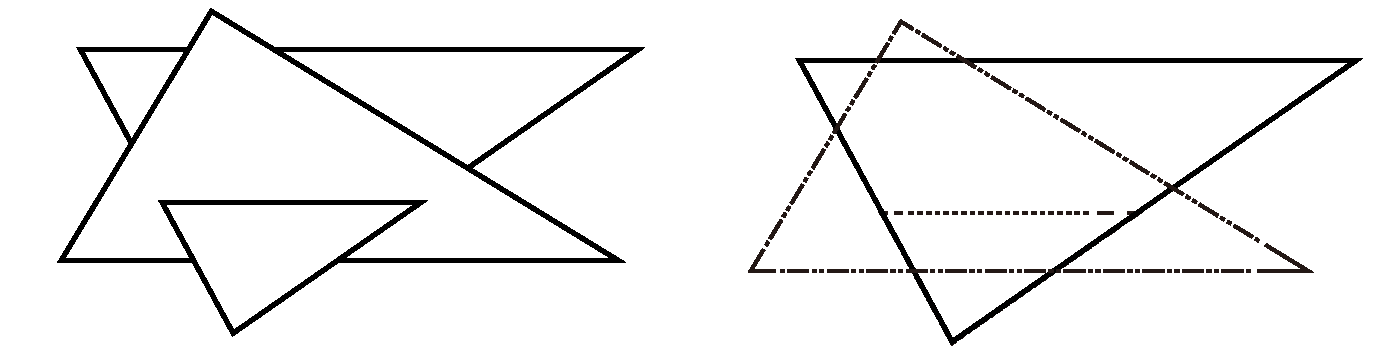
\includegraphics[width=3.5in]{edgeisect}
\caption{Different conditions of edge intersection. Triangle faces $t_1$ and $t_1^*$ are companion faces. Triangle faces $t_2$ and $t_2^*$ are companion faces. a) $t_2$ and $t_2^*$ are on different sides of $t_1$. b) $t_2$ and $t_2^*$ are on the same side of $t_1$. c) $t_2^*$ is coplanar with $t_1$. d) Both $t_1$ and $t_2$ have companion faces: the intersection is an edge intersection for both $t_1$ and $t_2$ (instead of only for $t_2$ is the previous three conditions). }
%Different conditions of edge intersection.
\label{fig:twin}
\end{figure}


\subsubsection{Copalnar}

\begin{figure}[t]
\centering
\includegraphics[width=3.5in]{boolean-03}
\caption{a) Coplanar cases; $t_1$ and $t_2$ intersect in 2D, dividing each other into two areas---a convex overlapping area and exclusive areas. b) Possible configurations of the companion faces. The blue triangles originate from the same mesh. For $\mathcal{I}_a$, the companion triangle $t_a$ is coplanar with $t_1$. Therefore, the overlapping areas ($t_1 \cap t_a$ and $t_1 \cap t_2$) do not need to be split by the yellow edge during tessellation, thus $\mathcal{I}_a$ is invalid. For $\mathcal{I}_b$ and $\mathcal{I}_c$, the companion faces are not coplanar, so these intersections can be recorded during an intersection test between $t_1$ and $t_a$ or $t_1$ and $t_b$. There is no need to record the intersection between $t_1$ and $t_2$.}
%Fig. 8. a) Coplanar cases; t1 and t2 intersect in 2D, dividing each other into two areas��a convex overlapping area, and exclusive areas.
\label{fig:coplanar}
\end{figure}

%Consider two triangle faces $t_1\in M_x$ and $t_2 \in M_y$ intersect within a common plane. Both $t_1$ and $t_2$ will divide each other into two areas---a convex overlapping area and exclusive parts (Fig. \ref{fig:coplanar}a). Apparantly, if we tessellate both $t_1$ and $t_2$ according to the boundary of overlapping area, we can guarantee that the tessellated meshes are intersection-free. Many previous methods \cite{feito2013fast,zhou2016mesh} use this method to guarantee topology correctness. However, in our method, we do not test whether $t_1$ and $t_2$ really intersect in 2D once we find they are coplanar. We treat coplanar situations as they do not intersect at all. In this way, we simplify our method, making it more robust and fast, while doing no harm to the topology correctness.

Consider two triangle faces,  $t_1\in M_x$ and $t_2 \in M_y$, which intersect within a common plane. Both $t_1$ and $t_2$ divide each other into two areas��a convex overlapping area and exclusive areas (Fig. \ref{fig:coplanar}a). If we tessellate both $t_1$ and $t_2$ according to the boundary of the overlapping area, we can guarantee that the tessellated meshes are intersection-free. Many previous methods \cite{feito2013fast,zhou2016mesh} use this process to guarantee topological correctness. However, in our method, we do not test whether $t_1$ and $t_2$ really intersect in 2D once we determine that they are coplanar. We treat coplanar situations as if they do not intersect at all. In this way, we simplify our method, making it faster and more robust, while having no effect on the topological correctness.

%We find that each intersection line segment in 2D is part of the edges from input meshes. That means we can view 2D intersection as a special case of edge intersection. The only difference is that there can be up to three edge intersections in one 2D intersection (red and yellow line segments in Fig. \ref{fig:coplanar}b). As we have discussed, edge intersection will be detected twice. That means we can rely on the companion triangle faces to detect intersections.

We find that each intersecting line segment is part of the edges of the input meshes in 2D. That means that we can view 2D intersections as special cases of edge intersections. However, there can be up to three edge intersections in one 2D intersection (red and yellow line segments in Fig. \ref{fig:coplanar}b). As discussed, edge intersections will be detected twice. Hence, we can rely on the faces of the companion triangles to detect intersections.

%However, if the companion triangles are also coplanar, neither of the two triangles will record the intersection. Fortunately, in this case, the intersection is not valid. The word `valid` means the intersections will appear as an edge in the final mesh, thus is necessary to put into tessellation. Supposing the intersection $\mathcal{I}$ is on $t_1$, this definition equals to:

However, if the companion triangles are also coplanar, neither of the two tests will detect the intersection. Fortunately, the intersection is not necessary in this situation. The neighboring faces of the intersection are all within the same plane. If the intersection is on the surface of the final mesh, the surface in the neighborhood of the intersection is a plane. Therefore, the intersection is not necessary to be an edge in the final model.

Because we do not process coplanar intersections, the coplanar areas may have different tessellations in different primitives. It seems that inconsistent topology can occur in the final mesh. In fact, all of the faces in a coplanar area has the same inclusion label vector, thus are collected or abandoned together. Therefore, if the coplanar area is on the surface of the final mesh, the coplanar area will have exactly the same tessellation as one of these primitives. This strategy will result in simpler topology than forcing the final tessellation to be consistent with all of the primitives.
